\documentclass[12pt]{article}
\usepackage{geometry}                % See geometry.pdf to learn the layout options. There are lots.
\geometry{letterpaper}                   % ... or a4paper or a5paper or ... 
%\geometry{landscape}                % Activate for for rotated page geometry
\usepackage[parfill]{parskip}    % Activate to begin paragraphs with an empty line rather than an indent
\usepackage{daves,fancyhdr,natbib,graphicx,dcolumn,amsmath,lastpage,url}
\usepackage{amsmath,amssymb,epstopdf,longtable}
\usepackage[final]{pdfpages}
\usepackage{paralist}  % need to modify standard enumerate blocks
\usepackage{tabto}
\newcommand\mytab{\tabto{1cm}}
\DeclareGraphicsRule{.tif}{png}{.png}{`convert #1 `dirname #1`/`basename #1 .tif`.png}
\pagestyle{fancy}
\lhead{CE 3354 -- Engineering Hydrology}
\rhead{FALL 2025}
\lfoot{ES9}
\cfoot{}
\rfoot{Page \thepage\ of \pageref{LastPage}}
\renewcommand\headrulewidth{0pt}



\begin{document}
\begin{center}
{\textbf{{ CE 3354 Engineering Hydrology} \\ {Exercise Set 9}}}
\end{center}

\section*{\small{Exercises}}

\begin{enumerate}
\item Figure \ref{fig:WasteCell} is a plan view of a waste cell at a solid waste disposal site.  Two borings are completed in the water table aquifer underlying the disposal site property. 
\begin{figure}[h!] %  figure placement: here, top, bottom, or page
   \centering
   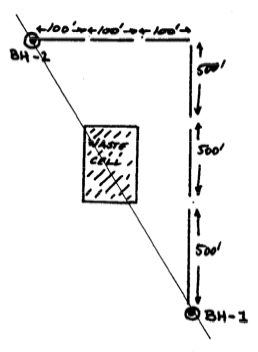
\includegraphics[width=2.0in]{WasteCell.png} 
   \caption{Plan View of an Waste Disposal Cell }
   \label{fig:WasteCell}
\end{figure}

The ground surface elevation at borehole BH-1 is 263.75 ft.  The ground surface elevation at borehole BH-2 is 249.75 ft.  The water table elevation in borehole BH-1 is 223.25 ft.  The water table elevation in borehole BH-2 is 229.75 ft.  The soil types in the area are silty-clay with a 
hydraulic conductivity of $K=3 \times 10^{-5}~\frac{ft}{sec}$ and an effective porosity of $n=0.40$.
A 100 x 500 foot waste cell is located between the two boreholes as shown. The bottom of the waste cell must be at least 5 feet above the water table.

Determine:
    \begin{enumerate}[a)]
        \item The hydraulic gradient (magnitude) from the provided information.
        \item The direction of groundwater flow from the provided information.
        \item The average linear (pore) velocity of groundwater.
        \item The minimum allowable elevation of the bottom of the waste cell.
        \item The anticipated travel time for contaminated leachate to reach the downstream borehole if the waste cell liner fails.
    \end{enumerate}

\clearpage
%%%%%%%%%%%%%%%%%%%%%%%%%%%%%%%
\item Figure \ref{fig:HorizontalAquifer} is a contour map of head in an aquifer system. 
\begin{figure}[h!] %  figure placement: here, top, bottom, or page
   \centering
   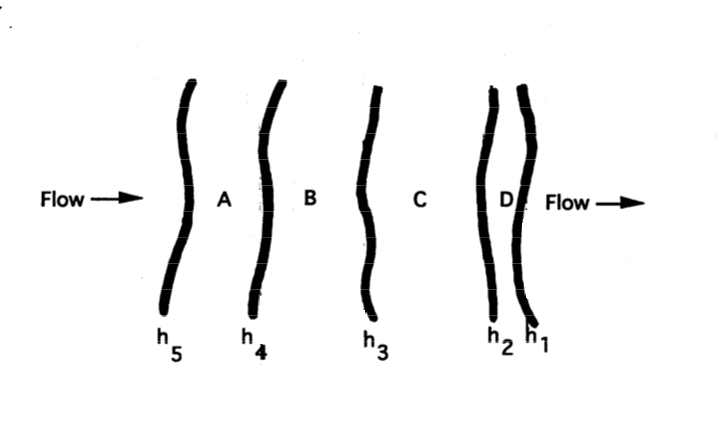
\includegraphics[width=5in]{PlanViewHeads.png} 
   \caption{Elevation View of an Aquifer }
   \label{fig:HorizontalAquifer}
\end{figure}

The aquifer medium is isotropic and inflow equals outflow.
The hydraulic conductivity of area A is $K=1 \times 10^{-6}~\frac{m}{sec}$

Determine:
    \begin{enumerate}[a)]
        \item The hydraulic conductivity in area B
        \item The hydraulic conductivity in area C
        \item The hydraulic conductivity in area D
    \end{enumerate}

\clearpage
%%%%%%%%%%%%%%%%%%%%%%%%%%%%%%%%%%%%%%%%%%%%%%%%%%%
\item Figure \ref{fig:VerticalAquifer} is a profile (elevation) view of an aquifer system. 
\begin{figure}[h!] %  figure placement: here, top, bottom, or page
   \centering
   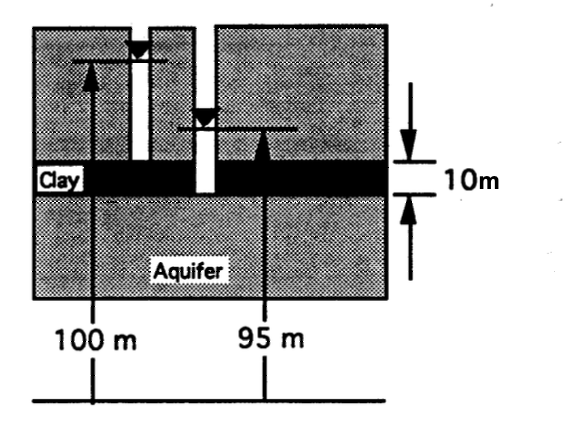
\includegraphics[width=5in]{VerticalAquifer.png} 
   \caption{Elevation View of an Aquifer }
   \label{fig:VerticalAquifer}
\end{figure}

The vertical hydraulic conductivity of the clay layer is $K_v=1 \times 10^{-7}~\frac{cm}{sec}$

Determine:
    \begin{enumerate}[a)]
        \item The distance (in meters) from the datum to the water level in the left piezometer.
        \item The distance (in meters) from the datum to the water level in the right piezometer.
        \item The vertical hydraulic gradient in the clay layer.
        \item The specific discharge across the clay layer in cm/sec.
        \item The direction of leakage.
    \end{enumerate}

\clearpage
%%%%%%%%%%%%%%%%%%%%%%%%%%%%%%%%%%%%%%%%%%%%%%%%%
\item Table \ref{tab:ThreeWell} is a list of observations of piezometric heads in three observation wells that penetrate the same homogeneous, isotropic, confined aquifer of thickness $B=20~m$

\begin{table}[h!]
\centering
\caption{Noname USA Aquifer Data}
\begin{tabular}{p{1.0in}p{1.5in}p{1.5in}p{1.0in}} % Column formatting, @{} suppresses leading/trailing space
~&~\\
Well ID & Easting (m) & Northing (m) & Head (m) \\
\hline
\hline
LJ-65-21-226 & 100.0  &  110.0 & 12.0 \\
LJ-65-21-227 & 400.0 &  100.0 & 13.5 \\
LJ-65-21-228 & 100.0 &  310.0 & 10.4 \\
\hline
\end{tabular}
\label{tab:ThreeWell}
\end{table}

Drilling cuttings from the wells indicate that the effective porosity is $n=0.20$, the hydraulic conductivity is $K=15~\frac{m}{day}$.  The piezometric surface between the wells can be approximated as a plane.

Determine:
    \begin{enumerate}[a)]
        \item The hydraulic gradient indicated by the data (magnitude and direction).
        \item The discharge in the aquifer per unit width.
        \item The average pore velocity at point P=(200,200).
    \end{enumerate}

\clearpage

%%%%%%%%%%%%%%%%%%%%%%%%%%%%%%%%%%%%%%%%%%%%%%%%%%%
\item Table \ref{tab:SomewhereUSAAquifer} is a list piezometric heads measured simultaneously in 13 wells penetrating an isotropic confined aquifer of thickness $B=50~m$, hydraulic conductivity $K=20~\frac{m}{day}$, and effective porosity $n=0.23$. 

\begin{table}[h!]
\centering
\caption{Somewhere USA Aquifer Data}
\begin{tabular}{p{1.0in}p{1.5in}p{1.5in}p{1.0in}} % Column formatting, @{} suppresses leading/trailing space
~&~\\
Well ID & Easting (m) & Northing (m) & Head (m) \\
\hline
\hline
MW-01 & 4300  &  1000 & 34.6 \\
MW-02 & 16500 &  3500 & 35.1 \\
MW-03 &  7000 &  5100 & 32.8 \\
MW-04 &  3000 &  6500 & 32.1 \\
MW-05 & 11000 &  7000 & 31.5 \\
MW-06 & 22000 &  6500 & 34.5 \\
MW-07 &  8000 &  9000 & 33.3 \\
MW-08 &  3200 & 11800 & 34.4 \\
MW-09 & 18100 & 10000 & 34.3 \\
MW-10 & 13500 & 12900 & 35.2 \\
MW-11 &  4000 & 15500 & 35.2 \\
MW-12 &  8700 & 16100 & 37.3 \\
MW-12 & 19500 & 16300 & 36.3 \\
\hline
\end{tabular}
\label{tab:SomewhereUSAAquifer}
\end{table} 

Determine:
    \begin{enumerate}[a)]
        \item A contour map of the head distribution (1-meter contour intervals)
        \item Specific discharge (direction and magnitude) at location $A=(10000,4000)$
        \item Specific discharge (direction and magnitude) at location $B=(16000,11000)$
        \item An estimate of total flow through the aquifer between wells MW-10 and MW-9.
        \item An estimate of travel time for a conservative tracer introduced near well MW-12 to reach MW-5
    \end{enumerate}

\clearpage







\end{enumerate}

\end{document}  